% Provenance (never printed): see sources/outline_sources.md (Year 1:
% the Solar System, planetology). Kepler's laws, the moment of inertia and
% the Stefan--Boltzmann law are owned by the physics series and recalled
% here; the equilibrium temperature and the Bond albedo are re-founded from
% Book 2 grade 10. Curves computed in figdata/bachelor-1/planet_table.py;
% numbers of the exercises and problem in the Book 3 scratch calculator
% ch03.py.
\chapter{علم الكواكب المقارن}\label{ch:b1:comparative-planetology}

تكاد الزهرة والأرض تكونان توأمين: فنصف قطر الزهرة \qty{95}{\percent} من نصف قطر الأرض، وكتلتها \qty{81}{\percent} من كتلتها. ومع ذلك فللأرض محيطات وغلاف جوي من النيتروجين والأكسجين وألواح تتحرك، بينما تُخفي الزهرة تحت الغيوم سطحًا حرارته \qty{737}{K}، أشدّ حرارةً من أيّ فرن مطبخ، ويسحقه غلاف جوي من ثاني أكسيد الكربون ضغطه \qty{92}{bar}. أما المريخ، وهو نصف حجم الأرض، فله غلاف جوي رقيق بارد، وبراكين عملاقة وأخاديد، لكن لا ألواح تتحرك فيه. وأبعد من ذلك، المشتري وزحل من الهيدروجين والهيليوم في معظمهما؛ أما أورانوس ونبتون ففي معظمهما جليد الماء والميثان والأمونياك. ومقارنة الكواكب هي السبيل الوحيد لاختبار ما نظنّ أننا نعرفه عن الأرض: لماذا باطنها متطبّق، ولماذا مناخها معتدل، ولماذا وحدها لها تكتونية الصفائح. يزن هذا الفصل الكواكب ويقيسها، ويقرأ باطنها من كثافاتها ومن توزيع كتلتها، ويقارن درجات حرارتها وأغلفتها الجوية، وينتهي بالأقمار والأجرام الصغيرة التي تحفظ سجلّ شباب المجموعة الشمسية.
% ledger: nasa:venus, earth:Rmean, earth:mass, nasa:uranus-structure

\begin{recall}
تدور الكواكب حول الشمس على قطوع ناقصة، ومربّع دور تابعٍ يتناسب مع مكعب نصف محوره الأكبر (قانون كبلر الثالث، في كتاب الفيزياء للسنة الأولى، حيث يُعرَّف أيضًا عزم القصور الذاتي للجسم الصلب؛ وللكرة المنتظمة $I = \tfrac25MR^2$). والجسم الأسود يشعّ $\sigma T^4$ من كل وحدة مساحة (السنة الثانية). وقد وُصفت المجموعة الشمسية والكواكب الصخرية والعملاقة في الكتاب 1 (الصف 6)؛ أما الألبيدو \omterm{def:b1:comparative-planetology:equilibrium-temperature}{ودرجة حرارة التوازن} لكوكب فقد عُرفا في الكتاب 2 (الصف 10)، وأثر الدفيئة في الكتاب 1 (الصف 9).
\end{recall}

\begin{omfigure}
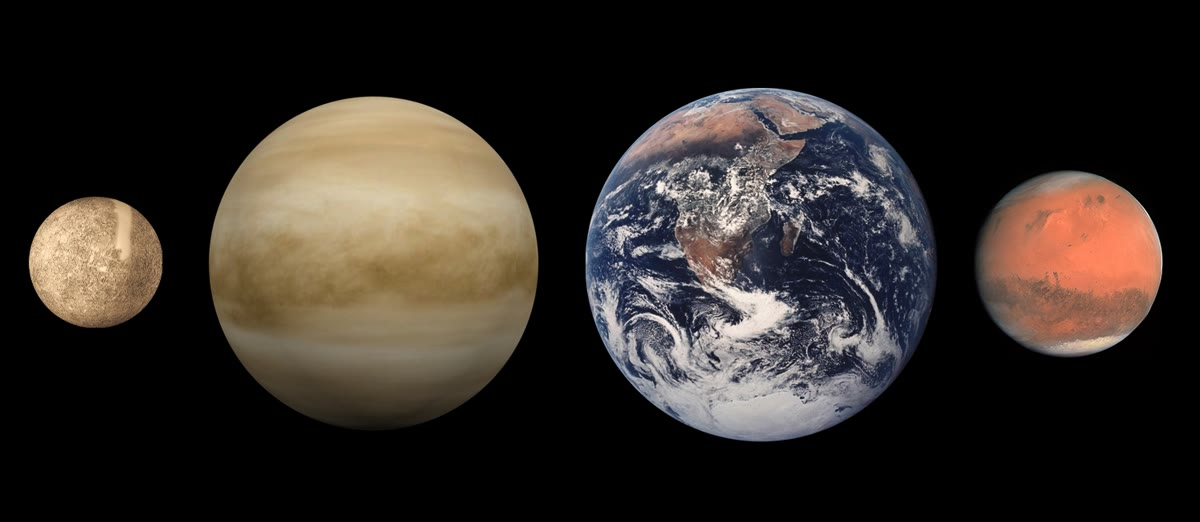
\includegraphics[width=0.85\linewidth]{images/book3/b1-terrestrial-planet-sizes.jpg}

{\small الكواكب الصخرية الأربعة بالمقياس، من اليسار إلى اليمين: عطارد والزهرة والأرض والمريخ (المسافات غير مرسومة بالمقياس؛ والزهرة كما تُرى في الضوء المرئي، وسطحها مخفيّ تحت الغيوم). NASA، في الملك العام.}
% ledger: commons:terrestrial-sizes
\end{omfigure}

\section{وزن الكواكب وقياسها}

يُقاس نصف قطر الكوكب من قطره الزاوي وبُعده، أو، لكوكب زارته مركبات فضائية، من قياسات الارتفاع بالرادار والليزر. أما كتلته فأصعب: إذ لا تُحسّ إلا بالجاذبية التي يمارسها على شيء آخر.

\begin{method}[كتلة الكوكب من مدار تابعه]\label{met:b1:comparative-planetology:mass}
من أجل تابع مهمل الكتلة على مدار شبه دائري نصف قطره (نصف المحور الأكبر) $a$ ودوره النجمي $T$ حول كوكب كتلته $M$:
\begin{enumerate}
  \item حوّل $a$ إلى أمتار و$T$ إلى ثوانٍ؛
  \item يعطي قانون كبلر الثالث $GM = 4\pi^2a^3/T^2$: هذا الجداء هو ما يقيسه المدار، وبدقة أكبر بكثير من $G$ نفسه؛
  \item اقسم على $G = \qty{6.6743e-11}{m^3.kg^{-1}.s^{-2}}$ لتحصل على $M$.
\end{enumerate}
ويُوزن كوكب بلا قمر (عطارد والزهرة) بالطريقة نفسها، من مدار مركبة فضائية تمرّ به أو من انحرافها.
\end{method}

\begin{example}
آيو، أقرب أقمار المشتري الكبيرة، يدور على $a = \qty{421.8e3}{km}$
في \num{1.769138} يومًا، أي $T = \qty{152854}{s}$. فيكون
\[
  GM = \frac{4\pi^2\times(\qty{4.218e8}{m})^3}{(\qty{152854}{s})^2}
  = \qty{1.268e17}{m^3.s^{-2}}, \qquad
  M = \frac{\num{1.268e17}}{\num{6.6743e-11}} = \qty{1.900e27}{kg},
\]
وهذا يوافق الكتلة الجدولية للمشتري، \qty{1.898e27}{kg}، بدقة \qty{0.1}{\percent}. أما كتلة آيو نفسها، أي \num{4.7e-5} من كتلة المشتري، فمهملة؛ والزيادة الصغيرة تأتي من انتفاخ المشتري الاستوائي، الذي يجذب قمرًا قريبًا أشدّ قليلًا مما تجذبه كرةٌ لها الكتلة نفسها.
% ledger: nasa:io, nasa:jupiter, const:G
\end{example}

ومع الكتلة ونصف القطر تأتي الكثافة المتوسطة $\bar\rho =
3M/(4\pi R^3)$، وهي أول دليل على ما يتكوّن منه الكوكب. وتتوزّع كثافات الكواكب في مجموعتين (انظر الشكل أدناه): فعطارد والزهرة والأرض والمريخ تقع بين نحو \num{3900} و\qty{5500}{kg.m^{-3}}، أي أكثف من أيّ صخر شائع؛ أما الكواكب الأربعة الخارجية فتقع بين \num{690} و\qty{1640}{kg.m^{-3}}، قرب كثافة الماء، وزحل أقلّ منه حتى.
% ledger: planet:Mercury.density, planet:Mars.density, planet:Earth.density, planet:Saturn.density, planet:Neptune.density

\begin{omfigure}
\begin{tikzpicture}
\begin{axis}[omrecord, width=0.86\linewidth, height=6.2cm, xmode=log,
  xmin=800, xmax=150000, ymin=0, ymax=6300, xlabel={\foreignlanguage{arabic}{نصف القطر الاستوائي \babelsublr{(\unit{km})}}},
  ylabel={\foreignlanguage{arabic}{الكثافة المتوسطة \babelsublr{(\unit{kg.m^{-3}})}}}, tick label style={font=\scriptsize},
  label style={font=\small}]
\addplot[only marks, mark=*, mark size=2.4pt, brown!70!black] table[x=R_km, y=density,
  restrict expr to domain={\thisrow{idx}}{0:2}] {figdata/out/bachelor-1-planet_table-bodies.dat};
\addplot[only marks, mark=*, mark size=2.4pt, brown!70!black] table[x=R_km, y=density,
  restrict expr to domain={\thisrow{idx}}{4:4}] {figdata/out/bachelor-1-planet_table-bodies.dat};
\addplot[only marks, mark=*, mark size=2.4pt, orange!85!black] table[x=R_km, y=density,
  restrict expr to domain={\thisrow{idx}}{5:6}] {figdata/out/bachelor-1-planet_table-bodies.dat};
\addplot[only marks, mark=*, mark size=2.4pt, omDef] table[x=R_km, y=density,
  restrict expr to domain={\thisrow{idx}}{7:8}] {figdata/out/bachelor-1-planet_table-bodies.dat};
\addplot[only marks, mark=o, mark size=2.4pt, black!60] table[x=R_km, y=density,
  restrict expr to domain={\thisrow{idx}}{3:3}] {figdata/out/bachelor-1-planet_table-bodies.dat};
\addplot[only marks, mark=o, mark size=2.4pt, black!60] table[x=R_km, y=density,
  restrict expr to domain={\thisrow{idx}}{9:9}] {figdata/out/bachelor-1-planet_table-bodies.dat};
\addplot[black!40, densely dashed] coordinates {(800,1000) (150000,1000)};
\begin{scope}[font=\scriptsize]
\node[left] at (axis cs:2439.5,5429) {عطارد};
\node[below left] at (axis cs:6052,5243) {الزهرة};
\node[above] at (axis cs:6378,5514) {الأرض};
\node[left] at (axis cs:3396,3934) {المريخ};
\node[left] at (axis cs:1737.5,3340) {القمر};
\node[right] at (axis cs:1188,1850) {بلوتو};
\node[above] at (axis cs:71492,1326) {المشتري};
\node[left] at (axis cs:60268,687) {زحل};
\node[right] at (axis cs:25559,1270) {أورانوس};
\node[above] at (axis cs:24764,1638) {نبتون};
\node[above left, black!60] at (axis cs:150000,1000) {الماء};
\end{scope}
\end{axis}
\end{tikzpicture}

{\small الكثافة المتوسطة بدلالة نصف القطر (بمقياس لوغاريتمي) للكواكب الثمانية (المملوءة: الصخرية، ثم العمالقة الغازية، ثم العمالقة الجليدية)، والقمر وبلوتو (دوائر مفرغة). بيانات ورقة الحقائق الكوكبية لناسا.}
% ledger: planet:Mercury.diameter, planet:Venus.diameter, planet:Earth.diameter, planet:Moon.diameter, planet:Mars.diameter, planet:Jupiter.diameter, planet:Saturn.diameter, planet:Uranus.diameter, planet:Neptune.diameter, planet:Pluto.diameter, planet:Mercury.density, planet:Venus.density, planet:Earth.density, planet:Moon.density, planet:Mars.density, planet:Jupiter.density, planet:Saturn.density, planet:Uranus.density, planet:Neptune.density, planet:Pluto.density
\end{omfigure}

لا تستطيع الكثافة المتوسطة وحدها أن تميّز كوكبًا مصنوعًا من مادة كثيفة واحدة من كوكب ذي مركز كثيف جدًا وغلاف أخفّ. أما العدد الثاني فيفعل ذلك: كيف تتوزّع الكتلة بين المركز والسطح.

\begin{definition}[عامل عزم القصور الذاتي]\label{def:b1:comparative-planetology:moi}
\emph{عامل عزم القصور الذاتي}\index{عامل عزم القصور الذاتي} للكوكب هو العدد
\[
  C = \frac{I}{MR^2} ,
\]
حيث $I$ عزم قصوره الذاتي حول محور دورانه، و$M$ كتلته، و$R$ نصف قطره المتوسط. والكرة المنتظمة لها $C = \tfrac25 = 0.4$؛ وكوكب تزداد كثافته نحو المركز له $C < 0.4$، وكلما تركّزت الكتلة أكثر كانت القيمة أصغر.
\end{definition}

يُقاس عزم القصور الذاتي من التمايل البطيء لمحور الدوران تحت جذب الشمس، مع تفلطح حقل جاذبية الكوكب. والقيم كاشفة: فالقمر، $C = 0.394$، شبه منتظم؛ والمريخ، $0.366$، والأرض، $0.3308$، طبقيّان بوضوح؛ والمشتري، $0.254$، وزحل، $0.210$، معظم كتلتهما متكدّس نحو مركزيهما.
% ledger: nasa:moon, nasa:mars, earth:MoI, nasa:jupiter, nasa:saturn

\section{ممَّ تتكوّن الكواكب}

\begin{definition}[الكواكب الصخرية والعمالقة]\label{def:b1:comparative-planetology:planet-types}
\emph{الكوكب الصخري}\index{الكوكب الصخري} كوكب يتكوّن في معظمه من صخور السيليكات والحديد، وله سطح صلب: عطارد والزهرة والأرض والمريخ. و\emph{الكوكب العملاق}\index{الكوكب العملاق} كوكب أكبر من الأرض بأضعاف كثيرة، يتكوّن في معظمه من عناصر خفيفة ومركّباتها، وليس له سطح صلب. و\emph{العملاق الغازي}\index{العملاق الغازي} كوكب عملاق يتكوّن في معظمه من الهيدروجين والهيليوم: المشتري وزحل. و\emph{العملاق الجليدي}\index{العملاق الجليدي} كوكب عملاق يتكوّن في معظمه من المركّبات التي يسمّيها الفلكيون جليدًا --- الماء والميثان والأمونياك --- تحت غلاف من الهيدروجين والهيليوم: أورانوس ونبتون.
\end{definition}

تؤكّد الأغلفة الجوية التي تقيسها المسابير والتلسكوبات هذا التقسيم. فغلاف المشتري من الهيدروجين بنسبة \qty{89.8}{\percent} ومن الهيليوم \qty{10.2}{\percent} بالحجم، وغلاف زحل \qty{96.3}{\percent} و\qty{3.25}{\percent}؛ أما أورانوس ففيه على الأقل \qty{80}{\percent} من الكتلة سائل حارّ كثيف من الماء والميثان والأمونياك فوق لبّ صخري صغير. وتبقى الكثافة المتوسطة لعملاق غازي منخفضة رغم أن مركزه مضغوط بشدة، لأن الهيدروجين أخفّ العناصر؛ \omterm{def:b1:comparative-planetology:planet-types}{والعملاق الجليدي} أكثف من زحل لأن جليده أثقل من الهيدروجين.
% ledger: nasa:jupiter, nasa:saturn, nasa:uranus-structure

والكواكب الصخرية طبقية كالأرض: لبّ غنيّ بالحديد تحت وشاح من السيليكات وقشرة رقيقة. وأبسط نموذج يستعمل العددين المقيسين، أي الكثافة المتوسطة \omterm{def:b1:comparative-planetology:moi}{وعامل عزم القصور الذاتي}، له طبقتان.

\begin{proposition}[الكوكب ذو الطبقتين]\label{prop:b1:comparative-planetology:two-layer}
نمذج كوكبًا نصف قطره $R$ بلبّ نصف قطره $xR$ وكثافته المنتظمة $\rho_c$ داخل وشاح كثافته المنتظمة $\rho_m$. وكثافته المتوسطة وعامل عزم قصوره الذاتي هما
\[
  \bar\rho = \rho_m + (\rho_c - \rho_m)\,x^3 , \qquad
  C = \frac25\,\frac{\rho_m + (\rho_c - \rho_m)\,x^5}{\bar\rho} .
\]
إذا عُرفت $\bar\rho$ و$C$ وفُرضت كثافة الوشاح $\rho_m$، فإن نصف القطر النسبي للّبّ يتبع من:
\[
  x^2 = \frac{\tfrac52C\bar\rho - \rho_m}{\bar\rho - \rho_m} ,
  \qquad \rho_c = \rho_m + \frac{\bar\rho - \rho_m}{x^3} .
\]
\end{proposition}

\begin{proof}
الكوكب كرة منتظمة كثافتها $\rho_m$ ونصف قطرها $R$، تُضاف إليها كرة نصف قطرها $xR$ بالكثافة الزائدة $\rho_c - \rho_m$. وتتجمّع الكتل:
$M = \tfrac43\pi R^3[\rho_m + (\rho_c - \rho_m)x^3]$، وبقسمة ذلك على الحجم نحصل على $\bar\rho$. وعزوم القصور الذاتي حول المحور نفسه تتجمّع كذلك؛ فكرة منتظمة كثافتها $\rho$ ونصف قطرها $r$ لها
$I = \tfrac25\cdot\tfrac43\pi\rho r^3\cdot r^2 = \tfrac{8\pi}{15}\rho r^5$،
فيكون $I = \tfrac{8\pi}{15}R^5[\rho_m + (\rho_c - \rho_m)x^5]$. وبقسمة $MR^2 = \tfrac43\pi\bar\rho R^5$ نحصل على $C$. وأخيرًا تُقرأ المعادلتان
$(\rho_c - \rho_m)x^3 = \bar\rho - \rho_m$ و$(\rho_c - \rho_m)x^5 =
\tfrac52C\bar\rho - \rho_m$؛ وبقسمة الثانية على الأولى نحصل على $x^2$، والأولى تعطي $\rho_c$.
\end{proof}

للنموذج ثلاثة مجاهيل ومعطيان، لذلك يجب فرض أحدها، وهو كثافة الوشاح، مما تزنه صخور التركيب المناسب تحت الضغط. والجواب حسّاس لهذا الاختيار حين تقترب $C$ من $0.4$، لأن $\tfrac52C\bar\rho - \rho_m$ تصبح فرقًا صغيرًا بين عددين كبيرين (\cref{exo:b1:comparative-planetology:10} والمسألة). ويهمل النموذج أيضًا ضغط الوشاح بوزنه الذاتي، وهو ما يرفع في كوكب بحجم الأرض كثافة الوشاح العميق كثيرًا فوق كثافة الصخور السطحية؛ أما بالنسبة إلى الأرض فالزلزال يفعل أفضل بكثير (\cref{ch:b1:layered-earth}). وقد فعلت مقاييس الزلازل المثبتة على المريخ الشيء نفسه لذلك الكوكب: فحيث يعطي الجدول الكوكبي نصف قطر لبّ قدره \qty{1830}{km}، تشير النتائج الحديثة إلى \qty{1650}{km} إلى \qty{1675}{km} فقط.
% ledger: nasa:mars-core

\begin{omfigure}
\begin{tikzpicture}[font=\scriptsize]
% scale: 0.5 cm per 1000 km
\fill[brown!35] (0,0) circle (3.1855cm);
\fill[orange!70!black] (0,0) circle (1.7425cm);
\draw (0,0) circle (3.1855cm);
  \node[align=center] at (0,0) {اللب\\ \qty{3485}{km}};
  \node[align=center] at (0,2.45) {الوشاح والقشرة};
  \node at (0,-3.55) {\small الأرض، $R = \qty{6371}{km}$};
\begin{scope}[xshift=5.6cm]
\fill[brown!35] (0,0) circle (1.6948cm);
\fill[orange!70!black] (0,0) circle (0.915cm);
\draw[white, densely dashed, thick] (0,0) circle (0.8313cm);
\draw (0,0) circle (1.6948cm);
  \node[align=center, white] at (0,0) {اللب};
  \node at (0,-2.1) {\small المريخ، $R = \qty{3389.5}{km}$};
  \draw[->] (1.25,1.75) node[above right, align=left] {الجدول: \qty{1830}{km};\\ المتقطّع: \qty{1650}{km}--\qty{1675}{km}} -- (0.62,0.62);
\end{scope}
\end{tikzpicture}

{\small الأرض والمريخ بالمقياس مع لبّيهما. في المريخ، الحافة الصلبة هي نصف قطر اللبّ في الجدول الكوكبي، والدائرة المتقطّعة هي النصف الأصغر الذي تشير إليه النتائج الزلزالية الحديثة. ولبّاهما غنيّان بالحديد؛ ولبّ الأرض له جزء داخلي صلب، غير مرسوم.}
% ledger: earth:Rmean, earth:Rcore, nasa:mars, nasa:mars-core
\end{omfigure}

\section{الأغلفة الجوية والأسطح}

تتحدّد حرارة الكوكب أولًا بضوء الشمس الذي يمتصه. والشدة الإشعاعية $S$ على بُعد $d$ من الشمس تتناقص مع $1/d^2$ (\cref{prop:b1:observing-the-sky:inverse-square}): \qty{1361}{W.m^{-2}} عند الأرض، و\qty{2601}{W.m^{-2}} عند الزهرة، و\qty{586}{W.m^{-2}} عند المريخ، و\qty{50}{W.m^{-2}} عند المشتري. ويرتدّ جزء منه مباشرةً إلى الخلف.
% ledger: earth:TSI, nasa:venus, nasa:mars, nasa:jupiter

\begin{definition}[ألبيدو بوند]\label{def:b1:comparative-planetology:albedo}
\emph{ألبيدو بوند}\index{ألبيدو بوند} $A$ لكوكب هو الكسر من القدرة الكلية لضوء الشمس الساقط عليه الذي يعكسه ويبعثره إلى الفضاء، عبر كل الأطوال الموجية وكل الاتجاهات.
\end{definition}

يعكس الثلج الطازج والغيوم الساطعة الكثير، ويعكس الصخر الداكن والبحر المفتوح القليل. والزهرة، المغلّفة بغيوم ساطعة، لها $A = 0.77$؛ والأرض $0.294$؛ والمريخ $0.250$؛ والقمر، وهو صخر رمادي داكن، $0.11$.
% ledger: nasa:venus, earth:albedo, nasa:mars, nasa:moon

\begin{definition}[درجة حرارة التوازن]\label{def:b1:comparative-planetology:equilibrium-temperature}
\emph{درجة حرارة التوازن}\index{درجة حرارة التوازن} $T_\mathrm{eq}$ لكوكب هي الحرارة المنتظمة التي يشعّ عندها جسم أسود بحجم الكوكب إلى الفضاء القدرةَ نفسها التي يمتصها الكوكب من الشمس بالضبط.
\end{definition}

\begin{proposition}[حساب درجة حرارة التوازن]\label{prop:b1:comparative-planetology:teq}
كوكب له \omterm{def:b1:comparative-planetology:albedo}{ألبيدو بوند} $A$ ويتلقى الشدة الإشعاعية $S$ يكون لديه
\[
  T_\mathrm{eq} = \left(\frac{S(1 - A)}{4\sigma}\right)^{1/4},
  \qquad \sigma = \qty{5.6704e-8}{W.m^{-2}.K^{-4}} .
\]
\end{proposition}

\begin{proof}
يعترض الكوكب ضوء الشمس الساقط على مقطعه العرضي، وهو قرص مساحته $\pi R^2$، ويمتص الجزء $1 - A$ منه: أي يمتص $S(1 - A)\pi
R^2$. أما جسم أسود (قانون ستيفان–بولتزمان، المقبول من كتاب الفيزياء للسنة الثانية) عند حرارة منتظمة $T$ فيشعّ $\sigma T^4$ من كل متر مربع من سطحه كله، $4\pi R^2$. وبمساواة القدرتين، $4\pi R^2\sigma T^4 = S(1 - A)\pi R^2$، والعامل 4 هو نسبة مساحة الكرة إلى مقطعها العرضي.
\end{proof}

بالقيم المذكورة أعلاه، تبلغ $T_\mathrm{eq}$ \qty{255}{K} للأرض، و\qty{227}{K} للزهرة، و\qty{210}{K} للمريخ، و\qty{270}{K} للقمر. والزهرة، مع أنها أقرب إلى الشمس، تخرج أبرد من الأرض: فغيومها تعكس ثلاثة أرباع ضوء الشمس. ويضع الشكل أدناه هذه القيم بجانب متوسطات الحرارة السطحية المقيسة. والفروق هي أثر الدفيئة، الذي تُكمله الفقرات التالية وفصول المناخ (\cref{ch:b1:radiation-heat-transport}) بالأرقام: نحو \qty{33}{K} للأرض، ونحو \qty{510}{K} للزهرة، ونحو \qty{4}{K} فقط للمريخ.
% ledger: const:sigma, earth:Tsurf, nasa:venus, nasa:mars, planet:Moon.Tmean

\begin{omfigure}
\begin{tikzpicture}
\begin{axis}[ybar, bar width=12pt, width=0.72\linewidth, height=5.8cm,
  ymin=0, ymax=820, xmin=-0.6, xmax=3.6, xtick={0,1,2,3},
  xticklabels={القمر,المريخ,الأرض,الزهرة}, ylabel={\foreignlanguage{arabic}{درجة الحرارة \babelsublr{(\unit{K})}}},
  tick label style={font=\scriptsize}, label style={font=\small},
  ymajorgrids, grid style={black!12}, axis lines*=left,
  legend style={font=\scriptsize, at={(0.03,0.97)}, anchor=north west, draw=none},
  nodes near coords, nodes near coords style={font=\tiny},
  every node near coord/.append style={/pgf/number format/fixed, /pgf/number format/precision=0}]
\addplot[fill=omDef!55, draw=omDef] table[x=idx, y=Teq] {figdata/out/bachelor-1-planet_table-temps.dat};
\addplot[fill=omThm!60, draw=omThm] table[x=idx, y=Tsurf] {figdata/out/bachelor-1-planet_table-temps.dat};
\legend{{درجة حرارة التوازن}, {متوسط الحرارة السطحية}}
\end{axis}
\end{tikzpicture}

{\small \omterm{def:b1:comparative-planetology:equilibrium-temperature}{درجة حرارة التوازن} (محسوبة من الشدة الإشعاعية \omterm{def:b1:comparative-planetology:albedo}{وألبيدو بوند}) ومتوسط الحرارة السطحية المقيسة لأربعة أجرام. يسخّن الغلاف الجوي الأرض، وفوق كل شيء الزهرة؛ ويكاد الغلاف الرقيق للمريخ لا يفعل شيئًا؛ والقمر، الذي لا غلاف له، أبرد في المتوسط من درجة حرارة توازنه.}
% ledger: nasa:moon, nasa:mars, earth:TSI, earth:albedo, earth:Tsurf, nasa:venus, planet:Moon.Tmean, const:sigma
\end{omfigure}

ومتوسط حرارة القمر، نحو \qty{253}{K}، يقلّ عن درجة حرارة توازنه. وهذا ليس لغزًا: فبلا غلاف جوي ولا محيط يحمل الحرارة، يكون جانب النهار شديد الحرارة وجانب الليل شديد البرودة، ولأن الإشعاع يتزايد مع $T^4$، فإن جسمًا غير متساوي الحرارة يشعّ القدرة الممتصة بمتوسط حرارة أدنى من جسم منتظم الحرارة (\cref{exo:b1:comparative-planetology:11}).

يفعل الغلاف الجوي أمرين: يترك معظم ضوء الشمس ينفذ، ويمتص جزءًا من الأشعة تحت الحمراء التي تبعثها الأرض فيعيد بعضها نحو الأسفل. ومقدار تدفئته للسطح يتوقف على كمية الغاز الماص فوق كل متر مربع. والضغط السطحي يقيس ذلك بالضبط: $p = mg$ لعمود كتلته $m$ لكل متر مربع. وغلاف الزهرة، عند \qty{92}{bar}، فيه \qty{96.5}{\percent} من ثاني أكسيد الكربون؛ أما غلاف المريخ، الذي لا يتجاوز \qty{6.36}{mbar} في المتوسط، ففيه \qty{95.1}{\percent} من ثاني أكسيد الكربون كذلك، لكنه يحمل نحو ستين مرة أقل من الغاز فوق كل متر مربع مما يحمله غلاف الأرض، وبخار ماء قليل جدًا. ولكلا الكوكبين غلاف من ثاني أكسيد الكربون؛ لكن أحدهما فقط غلافه سميك.
% ledger: nasa:venus, nasa:mars, earth:psurf

\begin{omfigure}
\begin{minipage}{0.4\linewidth}
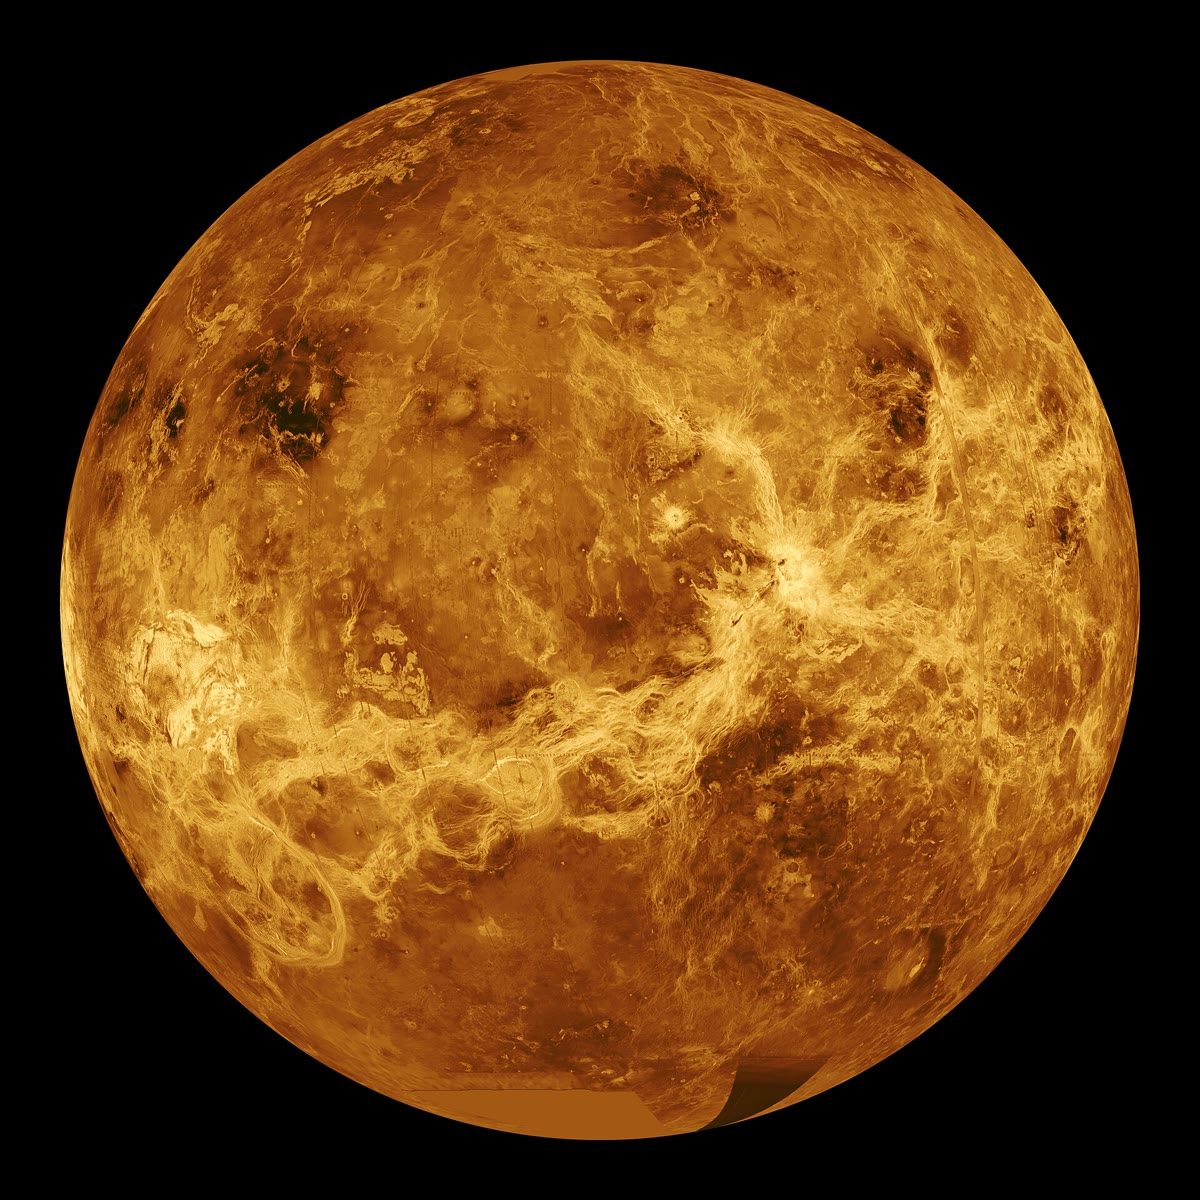
\includegraphics[width=\linewidth]{images/book3/b1-venus-radar-globe.jpg}
\end{minipage}\hspace{0.06\linewidth}
\begin{minipage}{0.4\linewidth}
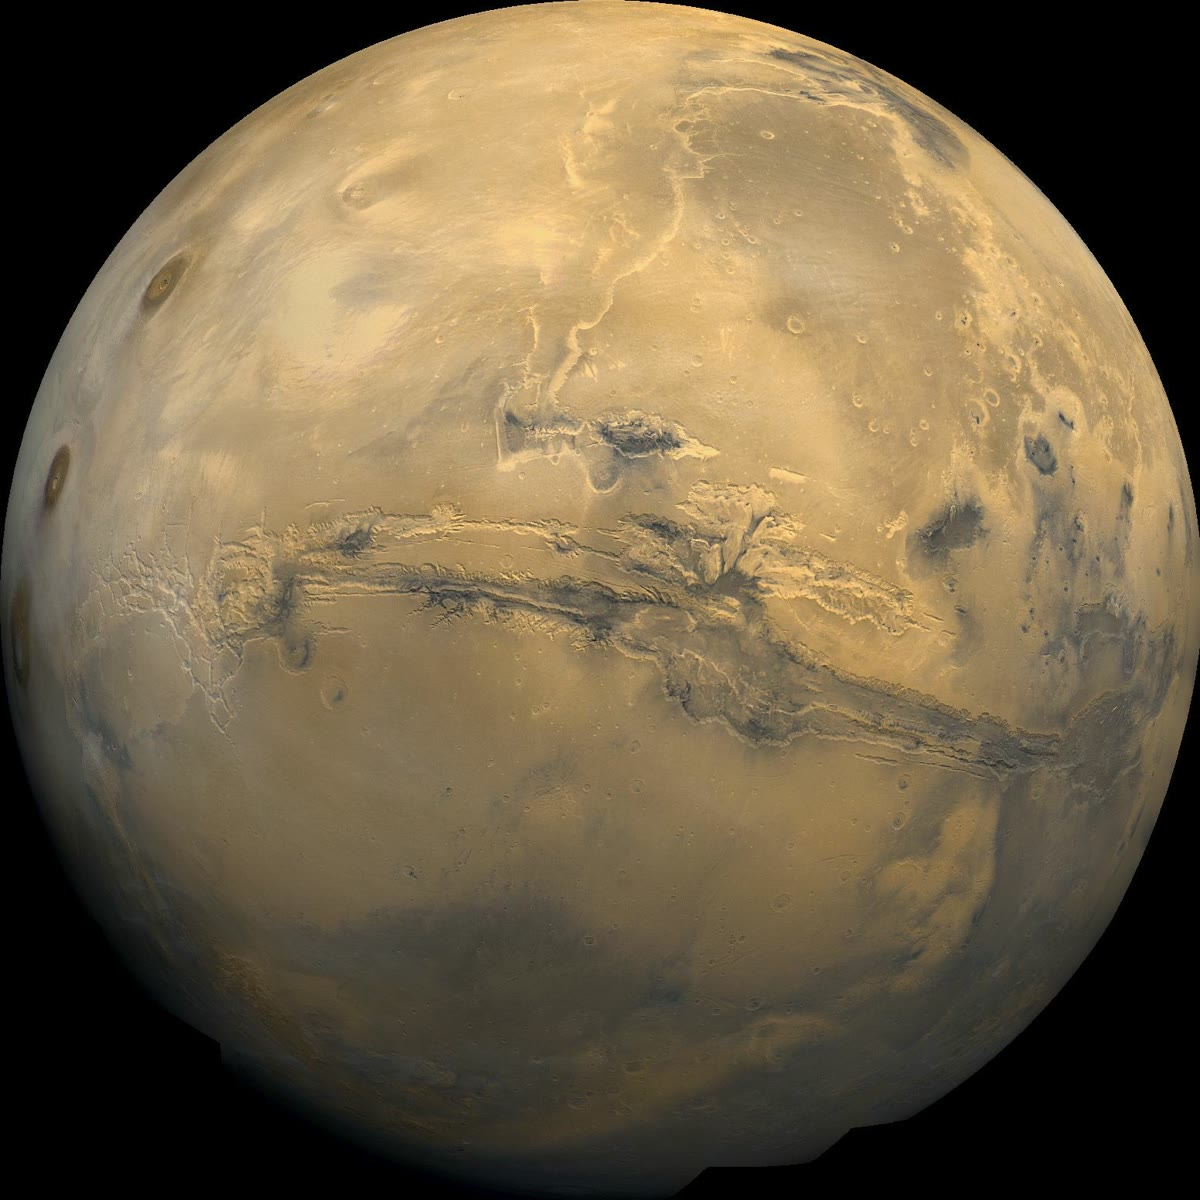
\includegraphics[width=\linewidth]{images/book3/b1-mars-valles-marineris.jpg}
\end{minipage}

{\small يسار: سطح الزهرة كما يُرى من خلال غيومها بالرادار لمركبة ماجلان، مُسقَطًا على كرة محاكاة حاسوبية (الألوان محاكاة). يمين: المريخ من المدار الفايكنغي 1، فسيفساء متمركزة على منظومة الأخاديد فاليس مارينيريس. NASA/JPL وNASA/USGS، في الملك العام.}
% ledger: commons:venus-globe, commons:mars-valles
\end{omfigure}

تحفظ الأسطح سجلّ ما شكّلها. فتتراكم الحفر الصدمية على كل سطح معرّض للفضاء، فالسطح المليء بالحفر، مثل معظم سطح القمر أو عطارد، قديم، والسطح القليل الحفر قد تجدّد: بتدفّقات الحمم، أو بالتعرية، أو بالصفائح التي تعيد قاع محيط الأرض إلى الوشاح. وتوجد السهول البركانية والبراكين على جميع الكواكب الصخرية. وتدل الصدوع والأخاديد والأحزمة المطوية على أن أغلفة الزهرة والمريخ الصخرية قد تشوّهت؛ لكن من بين الكواكب كلها لا تُظهر اليوم إلا الأرض غلافًا صخريًا مكسورًا إلى صفائح تتحرك ككتل صلبة، بظهرات حيث تتكوّن وخنادق حيث تغوص. ولا يزال يُناقش لماذا تنفرد الأرض بالتكتونية الصفائحية؛ ووجود الماء، الذي يُضعف الصخور، من الأسباب المطروحة.

\section{الأقمار والأجرام الصغيرة}

القمر، وقطره ربع قطر الأرض، كبير بالنسبة إلى تابع. وكثافته، \qty{3340}{kg.m^{-3}}، قريبة من كثافة صخور وشاح الأرض، وعامل عزم قصوره الذاتي، القريب من $0.4$، يدلّان على أنه لا يملك على الأكثر إلا لبًّا حديديًا صغيرًا. وللكواكب العملاقة منظومات من الأقمار هي عوالم قائمة بذاتها (انظر الصورتين أدناه). آيو، أقرب أقمار المشتري الكبيرة الأربعة، هو أكثر العوالم نشاطًا بركانيًا في المجموعة الشمسية، بمئات البراكين، يُسخَّن بالمدّ الذي يرفعه فيه المشتري؛ والبركانية تجدّد سطحه أسرع مما تستطيع الاصطدامات أن تعلّمه بحفر كبيرة. أوروبا، كثافتها \qty{3010}{kg.m^{-3}}، صخر تحت قشرة من الجليد، وثمة أدلة قوية على محيط مالح تحت تلك القشرة. وغانيميد وكاليستو، كثافتاهما \num{1940} و\qty{1830}{kg.m^{-3}}، مؤلفان من صخر وجليد بكميات متقاربة. تيتان، أكبر أقمار زحل، هو القمر الوحيد الذي له غلاف جوي كثيف، معظمه نيتروجين مع قليل من الميثان، وهو العالم الوحيد غير الأرض الذي له أنهار وبحيرات وبحار على سطحه --- من الميثان والإيثان السائلين؛ وهو يخفي على الأرجح محيطًا من الماء أيضًا.
% ledger: planet:Moon.diameter, planet:Earth.diameter, planet:Moon.density, nasa:moon, nasa:io-facts, nasa:europa, nasa:europa-facts, nasa:ganymede, nasa:titan-facts

\begin{omfigure}
\begin{minipage}{0.4\linewidth}
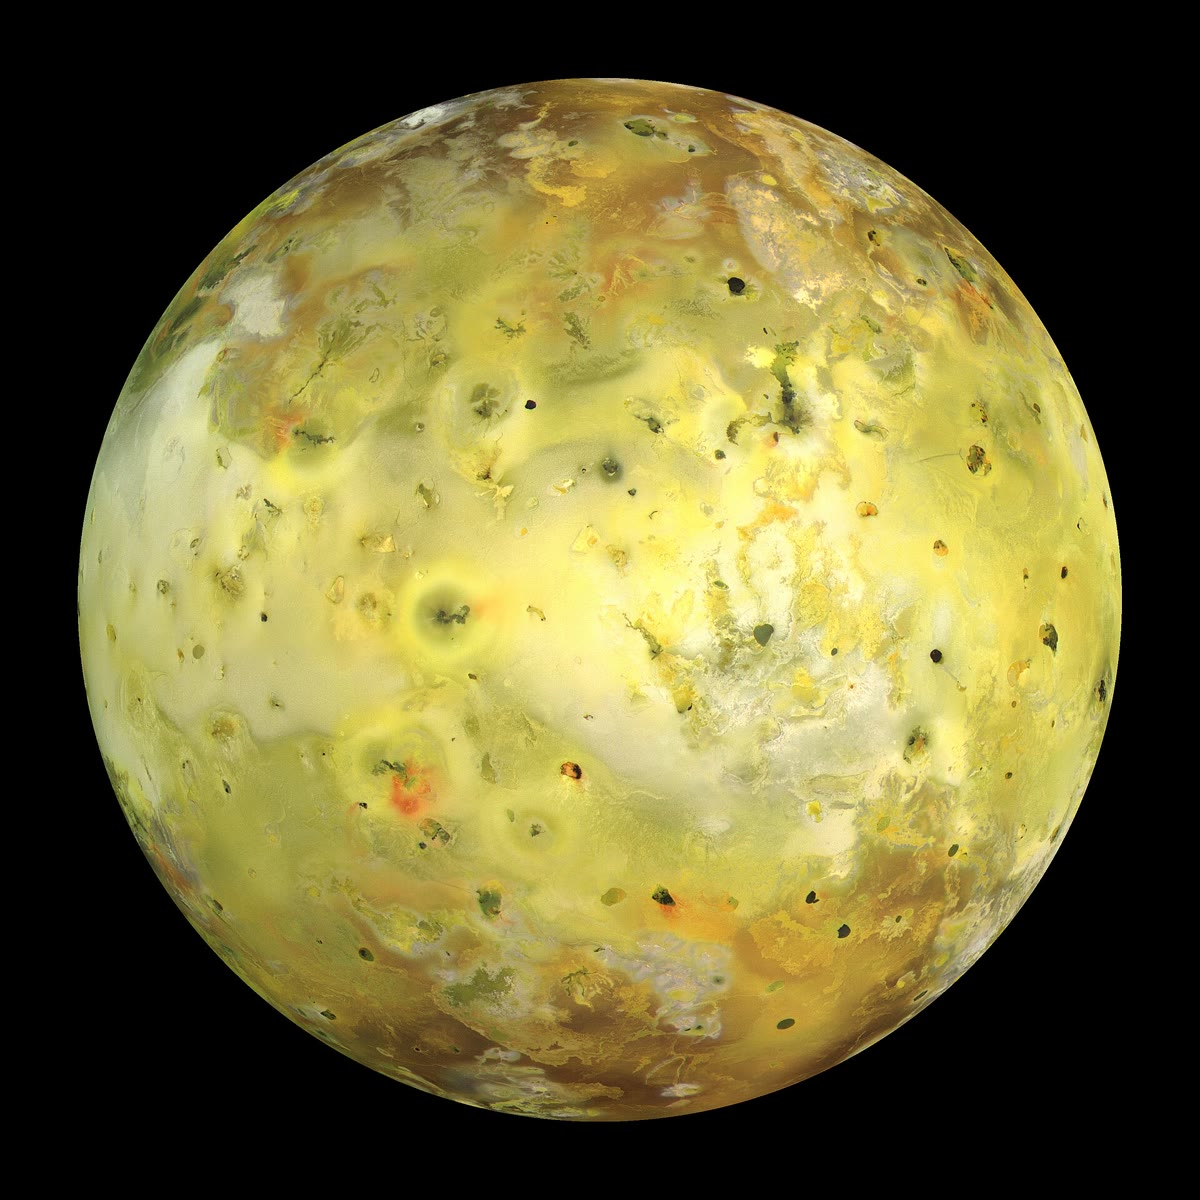
\includegraphics[width=\linewidth]{images/book3/b1-io.jpg}
\end{minipage}\hspace{0.06\linewidth}
\begin{minipage}{0.4\linewidth}
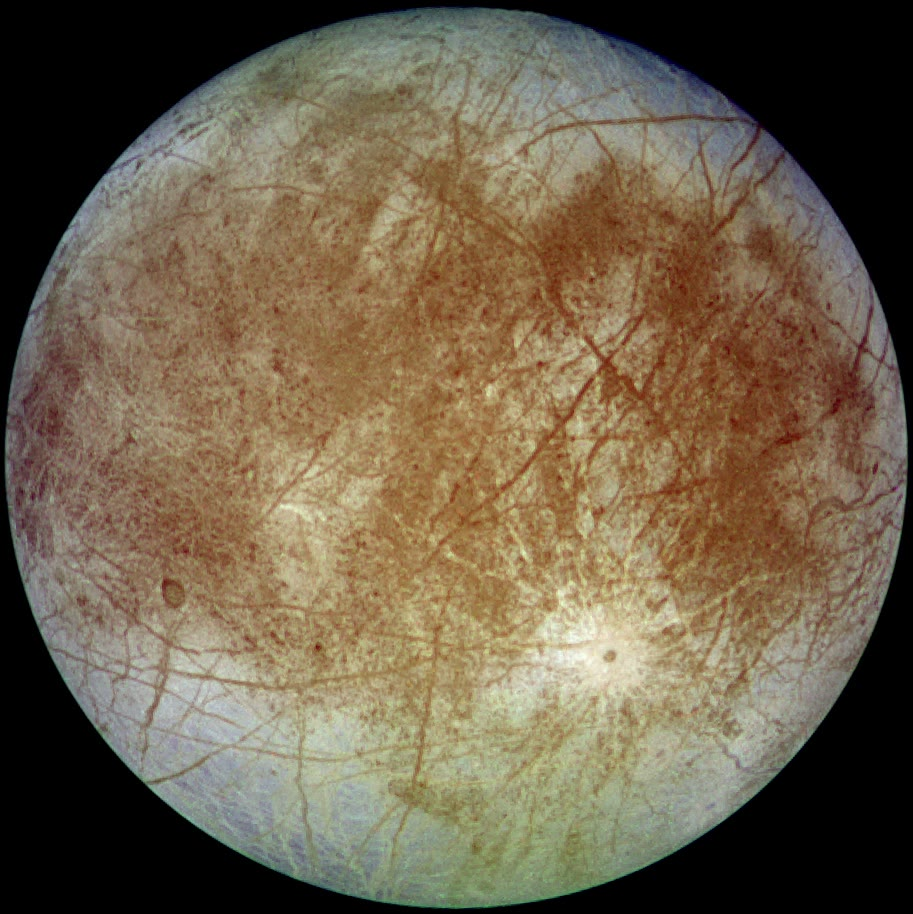
\includegraphics[width=\linewidth]{images/book3/b1-europa.jpg}
\end{minipage}

{\small قمران كبيران من أقمار المشتري، كما رصدتهما مركبة غاليليو. يسار: آيو، سطحه منقّط بمراكز بركانية، وملوّن بمركبات الكبريت والحمم. يمين: أوروبا بلون طبيعي تقريبي؛ والخطوط الداكنة الطويلة كسور في قشرتها الجليدية. NASA/JPL/جامعة أريزونا وNASA/JPL/DLR، في الملك العام.}
% ledger: commons:io, commons:europa, nasa:io-facts, nasa:europa
\end{omfigure}

\begin{definition}[الكويكب، والمذنب، والجرم عبر النبتوني]\label{def:b1:comparative-planetology:small-bodies}
\emph{الكويكب}\index{الكويكب} جرم صغير صخري أو معدني يدور حول الشمس، أصغر من أن يكون كوكبًا، وليس له غلاف الغاز والغبار الذي للمذنب؛ ومعظمها يدور بين المريخ والمشتري. و\emph{المذنب}\index{المذنب} جرم صغير من جليد وغبار، فإذا قرّبه مداره من الشمس أطلق غازًا وغبارًا يكوّنان حوله غلافًا متوهجًا وذيولًا تمتدّ مبتعدةً عن الشمس. و\emph{الجرم عبر النبتوني}\index{الجرم عبر النبتوني} جرم في المجموعة الشمسية يقع مداره، في المتوسط، خارج مدار نبتون.
\end{definition}

الأجرام عبر النبتونية في حزام كويبر، وهو منطقة على شكل قرص وراء نبتون، أجرام جليدية وصخرية بقيت من تكوّن الكواكب؛ وبلوتو، المصنّف كوكبًا قزمًا منذ 2006، واحد منها. والكويكبات بقايا منطقة لم يتكوّن فيها كوكب. وتسقط قطع من الكويكبات، وعدد قليل من قطع القمر والمريخ، على الأرض نيازك. وهي، إلى جانب ما أعادته المركبات الفضائية، العينات الوحيدة التي بين أيدينا لعوالم أخرى، وبعضها تغيّر قليلًا منذ تكوّن المجموعة الشمسية؛ أما أصنافها، وما تقوله عن تركيب الأرض وعن عمر المجموعة الشمسية، فموضوع الكتاب 2.
% ledger: nasa:pluto-facts

\section{التمارين}

\begin{exercise}[$\star$]\label{exo:b1:comparative-planetology:1}
للمشتري كتلة قدرها \qty{1898.13e24}{kg} ونصف قطر متوسط قدره \qty{69911}{km}. احسب كثافته المتوسطة وقارنها بكثافة الماء، \qty{1000}{kg.m^{-3}}.
\end{exercise}

\begin{exercise}[$\star$]\label{exo:b1:comparative-planetology:2}
باستعمال شكل الكثافات ونصف القطر، صنّف عطارد وزحل وأورانوس والزهرة بين الكواكب الصخرية أو العمالقة الغازية أو العمالقة الجليدية، وبرّر كل اختيار بنصف قطره وكثافته.
\end{exercise}

\begin{exercise}[$\star$]\label{exo:b1:comparative-planetology:3}
تتلقى الزهرة \qty{2601.3}{W.m^{-2}} ولها \omterm{def:b1:comparative-planetology:albedo}{ألبيدو بوند} قدره 0.77. احسب درجة حرارة توازنها. لماذا تقلّ عن درجة حرارة الأرض، مع أن الزهرة أقرب إلى الشمس؟
\end{exercise}

\begin{exercise}[$\star$]\label{exo:b1:comparative-planetology:4}
رتّب القمر ($C = 0.394$)، والمريخ (0.366)، والأرض (0.3308)، والمشتري (0.254)، وزحل (0.210) من الأكثر انتظامًا إلى الأكثر تركّزًا في المركز. ما قيمة $C$ لكوكب تتركّز كتلته كلها في نقطة عند مركزه؟
\end{exercise}

\begin{exercise}[$\star\star$]\label{exo:b1:comparative-planetology:5}
يدور تيتان حول زحل على $a = \qty{1221.87e3}{km}$ في \num{15.945421} يومًا. احسب كتلة زحل وقارنها بالكتلة الجدولية، \qty{568.32e24}{kg}.
\end{exercise}

\begin{exercise}[$\star\star$]\label{exo:b1:comparative-planetology:6}
تتلقى الأرض \qty{1361}{W.m^{-2}} على بُعد \qty{149.6e6}{km} من الشمس. احسب الشدة الإشعاعية عند المريخ (\qty{228.0e6}{km}) وعند المشتري (\qty{778.5e6}{km})، وقارنها بالقيمتين الجدوليتين \qty{586.2}{W.m^{-2}} و\qty{50.26}{W.m^{-2}}.
\end{exercise}

\begin{exercise}[$\star\star$]\label{exo:b1:comparative-planetology:7}
بيّن أنه عند ألبيدو معيّن تتغيّر $T_\mathrm{eq}$ وفق $d^{-1/2}$. احسب $T_\mathrm{eq}$ للمشتري ($S = \qty{50.26}{W.m^{-2}}$، $A = 0.343$). وإذا وُجد أن المشتري يشعّ قدرة أكبر من القدرة التي يمتصها من الشمس، فماذا يعني ذلك عن باطنه؟
\end{exercise}

\begin{exercise}[$\star\star$]\label{exo:b1:comparative-planetology:8}
احسب الاحترار الدفيئ $T_\mathrm{surf} - T_\mathrm{eq}$ للزهرة (\qty{737}{K})، وللأرض (\qty{288}{K}، $A = 0.294$)، وللمريخ (\qty{214}{K}). عبّر عن كل منها ككسر من $T_\mathrm{eq}$.
\end{exercise}

\begin{exercise}[$\star\star$]\label{exo:b1:comparative-planetology:9}
بالنسبة إلى كرة منتظمة، بيّن أن $C = 0.4$ بتكامل عزوم القصور الذاتي لقشور كروية رقيقة (لقشرة نصف قطرها $r$ وكتلتها $\mathrm dm$ عزم قصور $\mathrm dI = \tfrac23 r^2\,\mathrm dm$). ما القيمة التي تكون لقشرة مجوّفة نصف قطرها $R$؟
\end{exercise}

\begin{exercise}[$\star\star\star$]\label{exo:b1:comparative-planetology:10}
لعطارد $\bar\rho = \qty{5429}{kg.m^{-3}}$، و$C = 0.35$، ونصف قطر قدره \qty{2439.7}{km}. مع كثافة وشاح قدرها \qty{3300}{kg.m^{-3}}، استعمل نموذج الطبقتين لإيجاد نصف قطر لبّه، وكثافة لبّه، وكسر كتلته الموجود في اللبّ. ما الملاحَظ في عطارد؟
\end{exercise}

\begin{exercise}[$\star\star\star$]\label{exo:b1:comparative-planetology:11}
نمذج جرمًا بلا غلاف جوي، نصف نهاره عند حرارة منتظمة $T_1$ ونصف ليله عند $T_2$، يشعّان معًا القدرة الممتصة. (أ) بيّن أنه إذا كان $T_1^4 + T_2^4 = 2T_\mathrm{eq}^4$، فإن المتوسط $(T_1 + T_2)/2$ لا يتجاوز $T_\mathrm{eq}$، ولا يساويها إلا حين $T_1 = T_2$. (ب) بالنسبة إلى القمر، $T_\mathrm{eq} = \qty{270}{K}$؛ خذ $T_2 = \qty{100}{K}$. احسب $T_1$ والمتوسط.
\end{exercise}

\begin{exercise}[$\star\star\star$]\label{exo:b1:comparative-planetology:12}
للزهرة نصف قطر قدره \qty{6051.8}{km}، وجاذبية سطحية \qty{8.9}{m.s^{-2}}، وضغط سطحي \qty{92}{bar}. احسب كتلة غلافها الجوي، وقارنها بكتلة غلاف الأرض، \qty{5.1e18}{kg}، وبكتلة الزهرة، \qty{4.8673e24}{kg}. ماذا توحي المقارنة عن المكان الذي يُحتفظ فيه بثاني أكسيد الكربون الأرضي؟
% ledger: earth:Matm, planet:Venus.gravity, nasa:venus
\end{exercise}

\section{مسألة: وزن المريخ وسبر باطنه}

\begin{problem}[{مسألة نهاية الأسبوع --- كتلة المريخ من قمره، وكثافته وحرارته، وحجم لبّه}]
\label{pb:b1:comparative-planetology:1}
% ledger: nasa:phobos, nasa:mars, nasa:mars-core, const:G, const:sigma, earth:psurf, earth:gmean, planet:Mars.Prot, planet:Earth.density
% numbers computed in the scratch calculator calc/ch03.py from the rounded data
يدور فوبوس، القمر الأكبر للمريخ، على بُعد متوسط قدره \qty{9378}{km} من مركز المريخ في \num{0.31891} يومًا. وللمريخ نصف قطر متوسط \qty{3389.5}{km}، وفترة دوران \qty{24.6}{h}، وعامل عزم قصور ذاتي $C = 0.366$، \omterm{def:b1:comparative-planetology:albedo}{وألبيدو بوند} 0.250، وضغط سطحي متوسط \qty{6.36}{mbar}؛ ويتلقى \qty{586.2}{W.m^{-2}} من الشمس، ومتوسط حرارته السطحية نحو \qty{214}{K}. وكتلة فوبوس \qty{1.06e16}{kg}. خذ $G = \qty{6.6743e-11}{m^3.kg^{-1}.s^{-2}}$ و$\sigma = \qty{5.6704e-8}{W.m^{-2}.K^{-4}}$.

\medskip
\noindent\textbf{الجزء الأول --- وزن المريخ.}
\begin{enumerate}
  \item حوّل دور فوبوس إلى ثوانٍ.
  \item احسب $GM$ للمريخ.
  \item استنتج كتلة المريخ.
  \item هل من الصواب إهمال كتلة فوبوس؟
  \item احسب السرعة المدارية لفوبوس.
  \item قارن دور فوبوس بدوران المريخ. في أيّ اتجاه يعبر فوبوس سماء المريخ؟
\end{enumerate}

\medskip
\noindent\textbf{الجزء الثاني --- الكثافة والجاذبية.}
\begin{enumerate}[resume]
  \item احسب حجم المريخ.
  \item احسب كثافته المتوسطة، مقرّبةً إلى \qty{10}{kg.m^{-3}}.
  \item قارنها بكثافة الأرض، \qty{5514}{kg.m^{-3}}. أعطِ سببين لكون الأرض أكثف.
  \item احسب الجاذبية عند سطح المريخ.
  \item احسب سرعة الإفلات من سطح المريخ.
\end{enumerate}

\medskip
\noindent\textbf{الجزء الثالث --- الحرارة والغلاف الجوي.}
\begin{enumerate}[resume]
  \item احسب درجة حرارة توازن المريخ.
  \item قارنها بمتوسط الحرارة السطحية. ما مقدار الاحترار الدفيئ؟
  \item احسب كتلة الغلاف الجوي فوق كل متر مربع من المريخ، وقارنها بكتلة غلاف الأرض ($p = \qty{1014}{hPa}$، $g = \qty{9.82}{m.s^{-2}}$).
  \item احسب الكتلة الكلية لغلاف المريخ الجوي.
  \item غلاف المريخ الجوي فيه \qty{95}{\percent} من ثاني أكسيد الكربون، ومع ذلك فالاحترار الدفيئ فيه صغير. اقترح سببًا.
\end{enumerate}

\medskip
\noindent\textbf{الجزء الرابع --- لبّ المريخ.}
\begin{enumerate}[resume]
  \item ما قيمة $C$ لو كان المريخ منتظمًا؟ ماذا تخبرنا القيمة المقيسة؟
  \item اكتب الكثافة المتوسطة لمريخ ذي طبقتين بدلالة نصف القطر النسبي للبّ $x$، وكثافة الوشاح $\rho_m$، وكثافة اللبّ $\rho_c$.
  \item اكتب عامل عزم قصوره الذاتي بالمجاهيل نفسها.
  \item بيّن أن $x^2 = (\tfrac52C\bar\rho - \rho_m)/(\bar\rho - \rho_m)$.
  \item مع الكثافة المتوسطة في السؤال 8 و$\rho_m =
        \qty{3500}{kg.m^{-3}}$، احسب $x$ وكثافة اللبّ.
  \item ما الكسر من كتلة المريخ الموجود في لبّه؟
  \item كرّر السؤال 21 مع $\rho_m = 3450$ و\qty{3550}{kg.m^{-3}}. ماذا تستنتج عن دقة النموذج؟
  \item أعطِ نصف قطر لبّ المريخ من النموذج مع $\rho_m = \qty{3500}{kg.m^{-3}}$، وقارنه بقيمة الجدول الكوكبي، \qty{1830}{km}، وبالنتيجة الزلزالية الحديثة، \qty{1650}{km} إلى \qty{1675}{km}.
\end{enumerate}
\end{problem}
